The heuristics selected for this evaluation are formed around Lee's BNC index\cite{lee2003bnc}.  This selection was chosen because of their alignment to operationalisable, human-level metadata and the existence of multiple corpora with this level of annotation.



There are two main approaches to populating the corpus description using these heuristics: either read the seed corpus' contents and classify each data point, or read a list of metadata from an existing index.  The latter approach is used in this evaluation, since it is applicable to corpora with partially-missing data (such as the personal corpus data resulting from data gathering in Chapter~\ref{sec:personal}).

The accuracy of the classifiers listed here is responsible for minimising excess dispersion relative to the input corpus.  The nature of their residual error is also going to apply bias to the resulting data set.

Since many of these heuristics surround operationalising a corpus, a large body of research exists for classifying and extracting useful dimensions from texts.  The heuristics presented here are proof-of-concept only, and it is expected that the design of the heuristics used for a study is selected to match the theoretical basis of any analysis.

In most corpus designs, word count would be considered a measure of the size of the corpus (rather than a property of its constituents).  The method evaluated here is capable of retrieving IID (independent and identically distributed) samples at different levels, and demands a different selection of heuristics and metadata when operating at the word or sentence level.  Document level metadata are both high-level enough to be distributed for confidential corpora and descriptive enough to enable accurate retrieval (by contrast, word or part-of-speech frequencies would reveal much of the contents of the original corpus, which may not be desirable).  They are also aligned with storage and indexing, which are both often performed at the document level online.




\subsection{Audience Level}
The BNC User's Reference Guide~\cite[p. 14]{burnard1995users}
describes audience level thus:

\begin{quote}
\ldots{}a subjective assessment of the text's technicality or difficulty.
\end{quote}

This is expanded upon slightly by Lee~\cite[p. 68]{lee2001genres}, saying:

\begin{quote}
    \textsl{Audience level}, on the other hand, is an \textbf{estimate} (by the compilers) of the \textbf{level of difficulty} of the text, or the amount of background knowledge of its subject matter which is assumed.
\end{quote}

One approach to modelling this complexity is to use word lists such as those used in education, however, this is difficult to apply to such disparate topics without extensive compilation of such lists.  A simpler approach uses metrics computed from the morphology of words to form a readability score.  Such metrics are already widely used in word processing software and for designing documents for public consumption.


The classifier used for evaluation is based on the Flesch reading ease score\cite{flesch1948new}.  This score is widely used, easy to compute, and correlates with the simple `low/med/high' classification used in the BNC metadata:

$$
readability_{F} = 06.835 - 1.015 \left( \frac{\text{total words}}{\text{total sentences}} \right) - 84.6 \left( \frac{\text{total syllables}}{\text{total words}} \right)
$$




%plot(density(as.numeric(as.character(dat$readability))), main="BNC Flesch-Kincaid Readability Scores", xlab="Readability Score (bandwidth: 3.192)")

In order to establish the meaning of the BNC audience level categories in terms of this score, means were computed from the BNC world data.  These means, shown in Table~\ref{tab:evaluation:heuristics:fscore} (a reproduction of Table~\ref{tab:rebuilding:method:fscore}), were used by a simple classification algorithm that selects the category with the nearest mean value.  This na\"ive method yields the accuracy indicated in the `na\"ive acc.' column of Table~\ref{tab:evaluation:heuristics:fscore}, indicating that the readability score is not an ideal measure of the audience level.

%Readability ranks: 
% - med: 1651 items, mean = 55.44412267430666, sd = 12.76812426643693, var = 163.02499728317557
% - low: 664 items, mean = 62.95293871760397, sd = 14.424512199650604, var = 208.06655219786907
% - high: 820 items, mean = 47.70965585209567, sd = 12.445956325065204, var = 154.90182884543054
% - ---: 914 items, mean = 82.02288020623476, sd = 20.6424573733852, var = 426.111046412025
%Classifier error: 
% - med: 1239 / 1651 = (75.04542701393095%
% - low: 226 / 664 = (34.036144578313255%
% - high: 277 / 820 = (33.78048780487805%
% - ---: 914 / 914 = (100.0%
\begin{table}[h]
    \center
    \begin{tabular}{|c|c|c|c|}
        \hline 
        $\bar{readability_{F}}$ & BNC Audience level & Standard Deviation & na\"ive acc. \\
        \hline 
        63 & Low & 14.4 & 65.9\% \\
        55 & Med & 12.7 & 25.0\% \\
        47 & High & 12.4 & 66.3\% \\
        82 & (unclassified, speech) & 20.6 & - \\
        \hline
    \end{tabular}
    \caption{Target Flesch reading ease scores and their equivalent BNC categorisation.}
    \label{tab:evaluation:heuristics:fscore}
\end{table}




\begin{figure}[h]
    \centering
    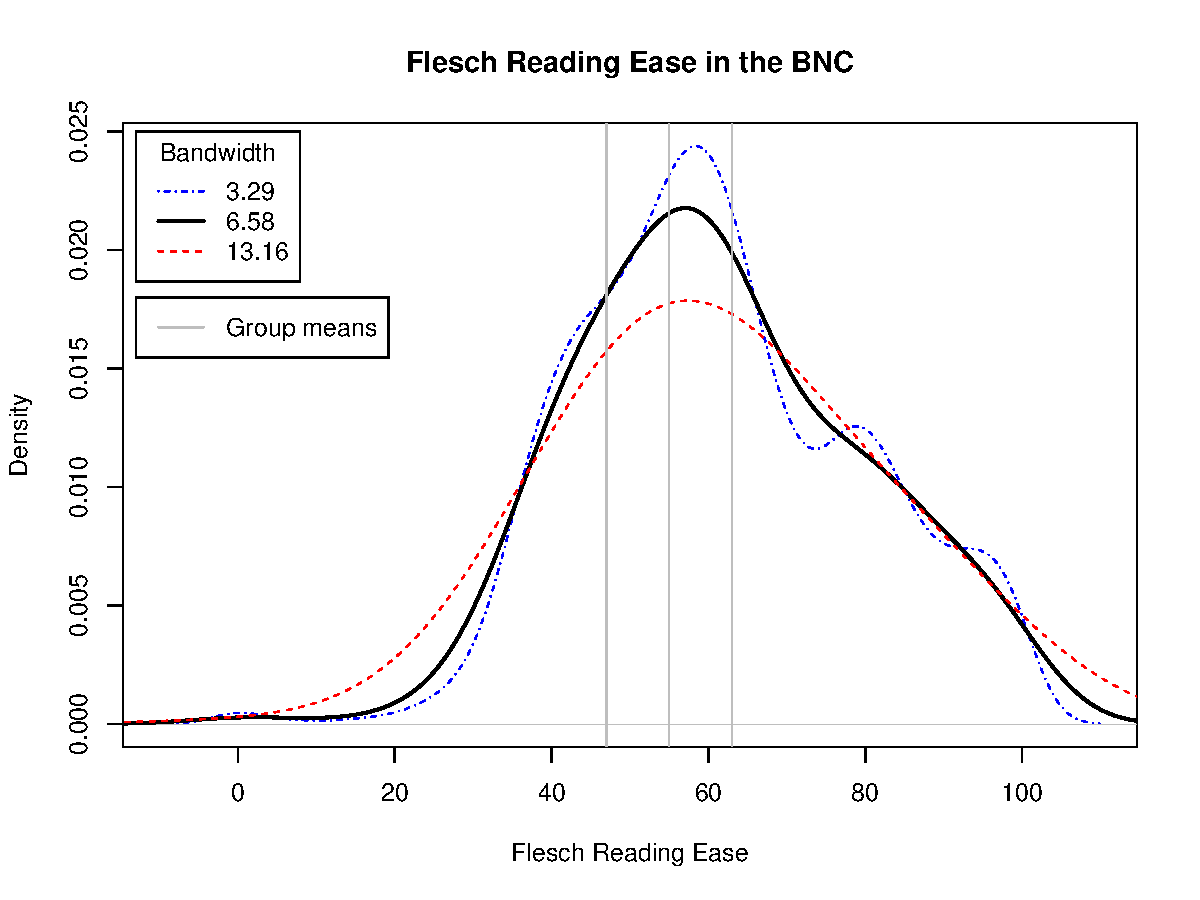
\includegraphics[width=0.8\textwidth]{evaluation/fleschbncdist}
    \caption{Flesch reading ease distribution in the BNC.}
    \label{fig:evaluation:heuristics:fleschbncdist}
\end{figure}


Rather than continue to use the categorisation used in the BNC, each text was scored for readability and the raw Flesch reading ease score used as its point within that dimension.  The `cpr' profiling tool then simply represents the underlying distribution as a continuous one (rather than artificially discretised into `high', `medium' and `low').

The standard deviation of categories within Table~\ref{tab:evaluation:heuristics:fscore} provides us with a convenient source for the bandwidth of the smoothing function used to identify the empirical distribution of the reading ease scores.  Using graphical methods (illustrated in Figure~\ref{fig:evaluation:heuristics:fleschbncdist}) the value of $\sigma / 2$ was chosen to represent the distribution: this offers a tradeoff between accurately portraying the distribution and permissively selecting documents online.  This method also clarifies the difficulties associated with attempting to accurately classify audience level based on readability metrics.

Where a text is unavailable, knowledge of the standard deviation of each of the readability categories in the BNC allows us to produce an approximation of the distribution of readability scores.  This approach (as well as the smoothing above) illustrates the value of manually modifying the text distributions during the design phase.

As we are using a proxy variable to impute the reading ease, any classifier accuracy issues are deferred to the assumption that `reading ease' is something we, as corpus designers, care about.






\subsection{Word Count}
Word counts are, for our purposes, trivial to compute.  There are two challenges to operationalising word counts, however.

The former of these pertains to metadata and other boilerplate within files.  Files must be processed prior to word counts being performed.  This means (like many other tools) that we must post-process candidate files even if we elect to discard their contents.

Secondly, it is necessary to normalise deviance measures when comparison documents: this poses a particular challenge as word counts are open-ended.  The method used here was to enforce an arbitrary limit, above which any distances in the word count dimension register as $1$.  Because the sampling method does not primarily rely on gradient descent, this is fairly safe, however, selection of the threshold does impact the importance assigned to word count (vs.\ some other metadata dimension): too high and it will undervalue differences in word count.

The arbitrarly limit selected for the BNC was $10,000$.  This is sufficiently large that any difference greater than it may be considered `absolute', that is, if there is a difference in length of over $10,000$ words, we can reasonably conclude that the lengths differ enough to be describing different texts.  In practice (as we shall discuss in Section~\ref{sec:evaluation:retrieval}) most documents fall short, and this limit could be reduced.

% --- 
It is worth noting the difference in philosophy this method embodies compared to many corpus studies: the word count here is a property of each document, and \textsl{not} a measure of corpus size.  Unlike many methods, we are sampling at the same level we are presuming analysis at.
% (though this level is variable due to the ease with which documents may be selected).






\subsection{Genre}
\label{sec:evaluation:heuristics:genre}
Genre is arguably the most important single stratification applied to a general-purpose corpus (even forming the bulk of the definition of its name), yet it remains one of the more nebulous terms.  Here we follow Lee's definitions once more, commensurate with the BNC index that serves as the source of much of the metadata for our corpus definition file.

Due to the complexity of genre taxonomies, and thus the relative difficulty of classifying documents therein, there is significant motive to take the same approach as audience level above: using a self-defined or simpler taxonomy to simplify imputation or selection.  On the other hand, the BNC classification is well-known and likely to be used in any corpus augmentation task (e.g. ``I want this subset of the BNC, but \textsl{more} of it.'').  We describe here an approach using the existing BNC classifications for this reason, with a discussion of the implications of other options below.


As this is a proof-of-concept system, the accuracy of the classifiers used need not be cutting-edge.  This relaxed requirement is reinforced by the notion that any errors are `sane', falling along such ambiguities as identified by Lee~\cite[p.~11]{lee2003bnc}:

\begin{quote}
It may be the case that the actual content/topic of these linguistics-related texts makes them seem less like social science texts than arts or applied science texts\ldots
\end{quote}

This `sanity of error' is enforced by using a distance measure that is based on rank correlation of token type frequencies, allowing two categories to be judged on a scale more meaningful than simple boolean equality.  This luxury may not be available for all potential discrete classification systems (such as those read from external indices), and is not a requirement of convergeance to the input distribution.

The distinction between genres is often somewhat variable: some, such as \variable{W\_newsp\_brdsht\_nat\_*}, are made between the subject of texts, whereas others fall along lines of context or what others may term `text type' (\variable{W\_email} vs. \variable{W\_essay\_sch}).  This makes it particularly difficult to identify a model that linearises features within the dataset consistently enough for many classification algorithms to work well.

Lee's taxonomy is partially hierarchical, with many of the more detailed categories harbouring both this `text type' distinction as well as one regarding topic.  Both were retained here as they align to two distinct processes when sampling: the text type is an indication of (roughly) where a document may be found, and the topic regards more which document to select.





% --

\paragraph{Classification}
The problem of identifying BNC genre from free text is a simple 70-way classification task\footnote{Such that a 70-way classification task may be described as simple at all.}.  In practice, the subjective nature of the taxonomy and the large number of classes makes this a challenging endeavour.  This is a clear illustration of the difficulties encountered using the ImputeCaT method: whilst it may not be necessary to find documents online with great accuracy, there must exist \textsl{some} method of discriminating between them in a useful way.



In his 2007 paper on web genres, Sharoff\cite{sharoff2007classifying}%
%p. 5
 fits a number of classifiers to the BNC, using a variety of genre taxonomies.  Therein he reports success using a supervised learning approach to classify `grouped' versions of the BNC taxonomy: one aligned to the EAGLES\cite{EagTcwgCtypeaglespreliminary} text typology recommendations, and one 10-way grouping based on unsupervised methods.

An alternative method would be to use entirely ground-up techniques such as factor analysis or LDA.  These mechanisms will extract maximally homogenous groupings from text, but at the expense of predictable alignment with human understanding (and thus any research questions or search engine designs).

Since part of the intent here is to retain a parsimonious corpus profile document, this heuristic makes use of the original categories from the BNC taxonomy.  Nonetheless, Sharoff's study was used as a starting point for the methodology, in line with the goal of using established methods for heuristics.

The ambiguity and external nature of some of the distinctions drawn in the BNC index causes problems here, and represents a common dichotomy in linguistics: a human-readable and intuitive classification is rarely easy to model quantitatively (to the point where we are often simply unable).

Ultimately, the classifiers detailed here used the na\"ive Bayes approach and were fit using WEKA\cite{hall2009weka}.  In accordance with the findings of McCallum \& Nigam, the multinomial model was used over the Bernoulli due to its ability to maintain classification accuracy in models with large numbers of dimensions\cite{mccallum1998comparison}.  This also unexpectedly yielded the benefit that it was much faster to fit.

For the use-case presented here, absolute accuracy of the classifier matters little: we care only that `positive'ly classified cases are reliable for any one pass over the set of candidate documents, \textsl{not} that every candidate is selected.  Because of this, and because the number of classes is high enough to indicate that errors are unlikely to occur in the direction of the current class, the evaluations below focus on the precision of each method.

As ever, the classifier performance reveals as much about the taxonomy of the input data as it does the classification method.  Presented here are six models that cover different subsets of the BNC:

\begin{itemizeTitle}
    \item[BNC70] A classifier built using all 70 categories of both written and spoken BNC portions.
    \item[BNC69a] This classifier omits \texttt{S\_conv}, which was deemed unreasonably general in its content and thus difficult to retrieve.
    \item[BNC69b] The BNC70 classifier, omitting \texttt{W\_misc} due to the breadth of said category.
    \item[BNC68] Omitting Both \texttt{W\_misc} and \texttt{S\_conv}.
    \item[BNC46] Written portions of the BNC, containing \texttt{W\_misc}.
    \item[BNC45] Written portions of the BNC, without \texttt{W\_misc}.
\end{itemizeTitle}

The decision to omit sections of the BNC was deemed a necessary trade-off to achieve functional performance: for the purposes of this evaluation, the actual subset used is only of importance to the generality of the results (rather than their veracity).  Likewise, the priority is not to produce a genre classifier, but merely to use one within the larger method: simply, it is more important that the classifier is functional than that it is general.

% Comparison of each model, with graphs.
\begin{table}[ht]
    \centering

    \begin{tabular}{|l|c|c|c|}
        \hline 
        Corpus & Accuracy & Precision & AUC \\
        \hline
        BNC45  &  70.7\%  &  0.721  &  0.901 \\
        BNC46  &  63.7\%  &  0.666  &  0.877 \\
        BNC68  &  71.5\%  &  0.715  &  0.913 \\
        BNC69a &  65.9\%  &  0.685  &  0.893 \\
        BNC69b &  72.1\%  &  0.732  &  0.918 \\
        BNC70  &  66.6\%  &  0.689  &  0.899 \\
        \hline
    \end{tabular}
    \caption{Weighted mean performance (per class) for each classifier.}
    \label{table:evaluation:heuristics:classifieraccuracy}
\end{table}

Table~\ref{table:evaluation:heuristics:classifieraccuracy} shows the resultant accuracy figures for the models trained on the BNC subsets mentioned.  10-way crossvalidation was used to estimate the above statistics, in an effort to reduce the potential for overfitting to a fixed test/training set.  The statistics are formed from a weighted mean of each classes performance against all others.

These figures reveal that {\textsl spoken conversation} (\texttt{S\_conv}) has the most deleterious effect on classifier accuracy, indicating that it overlaps most with other categories.  Whilst it was expected that \texttt{W\_misc} would also do this, the performance improvement shown in BNC69b over BNC68 indicates that \texttt{W\_misc} contains some distinct features that are best retained.  Though using a different design of classifier, overall performance is roughly in-line with Sharoff's BNC-based classifiers\footnote{Attempts to fit SVM-based models lead to lower performance than multinomial na\"ive Bayes.  I believe this to be a result of the high number of classes}\cite{sharoff2007classifying}.  The $45$- and $46$-class models are written-only equivalents, and are listed here due to their use in the retrieval task below.

    

\begin{figure}[Ht]
    \centering
    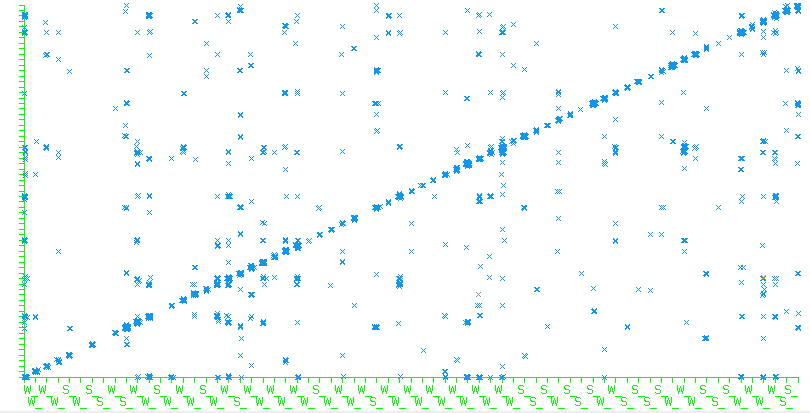
\includegraphics[width=1\textwidth]{evaluation/bnc68bconfusion}
    \caption{BNC68b confusion matrix}
    \label{fig:evaluation:heuristics:bnc68bconfusion}
\end{figure}



There are also potential arguments for the omission of many other categories from the taxonomy used here, however.  Figure~\ref{fig:evaluation:heuristics:bnc68bconfusion} shows the confusion matrix for the BNC69b classifier---note that some jitter has been applied to the plot to accentuate the overplotted items.  This shows a rough smattering of difficult-to-classify classes, though a more detailed inspection of the per-class tests on the model indicates that only two of these perform with AUC values below 0.7: \texttt{W\_fict\_drama} and \texttt{W\_essay\_univ}, which are classified in a way indistinguishable from chance.  Some classes with distinct lexical features (such as \texttt{W\_email} and \texttt{S\_sermon}) are classified particularly accurately.

The error surface described in Figure~\ref{fig:evaluation:heuristics:bnc68bconfusion} will contribute to the resulting error of the system, and as such further increase the variance of the output corpus.  Again, this is analogous to the coding stage of any conventional corpus building project, but with the distinct advantage that the propensity for classification error is well-known.  As shown, there are no instances where a genre is consistently mis-classified, indicating that errors will not systematically bias any output to a great degree.  The full accuracy data is presented in Appendix~\ref{sec:appx:bayesianbnc68}.

% -- 
\paragraph{}

One final note should cover the generality of the methods used here.  As with all portions of the heuristics, the choice of classifier is heavily theory-laden, and should conform to the underlying data's nature as much as possible.  Classification of genre is a particularly awkward aspect since it relies on imputing fairly complex external information (such that it can then be worked with by the software) from linguistic content, something that, as a rule, should be avoided for the sake of statistical validity.  Notably, the EAGLES guidelines on text typology\cite{EagTcwgCtypeaglespreliminary} warn:

\begin{quote}
The classification of texts into different genres seems to have been mostly achieved through external criteria rather than through internal, linguistic criteria.
\end{quote}

The manner of retrieval and the nature of the web offer some avenues for working with external data and closing this gap: It is firstly possible to retrieve documents according to an existing genre directory, all but guaranteeing a fit.  Further, HTML and HTTP metadata and stylistic properties of web documents (or those which are closely linked) may indicate genre as effectively (or more) as linguistic content.  These are all places where further research dovetails with the methods described here to increase overall accuracy.  Further work would be necessary to validate methods of reliably extracting and using this data, especially where it is patchy or difficult to extract.  Such efforts would prove particularly fruitful, however, where the seed corpus originates online, allowing the profiling and heuristic classification stages to operate using the same implementation.






